\chapter{Rover Implementation}
\lhead{\emph{Rover Implementation}}
\label{chapter:rover}

The aim of this project is the development of a VR teleoperations system. This necessitates the procurement of some form of robotic platform to demonstrate the system on. This platform must be easily modifiable and cheap enough to be within budget, so it was determined that the most logical solution was to design a simple rover for the project; this is both cheap and allows for complete customisation with minimal hassle. The internals of the rover are shown in Figure \textcolor{red}{[HARDWARE PICS]}, and a block diagram of the hardware in Figure \ref{fig:hardware}. Due to the rover being a simple test platform for the proposed system, its hardware is mostly irrelevant to this report and therefore will not be discussed in detail (a detailed breakdown can be found in Appendix \ref{appendix:hardware}). The application of computer vision techniques in an embedded system has high processing requirements, leading to the selection of a Raspberry Pi 3 as the core of the system (it was the highest performance embedded device readily available). 

\begin{figure}[H]
    \begin{center}
      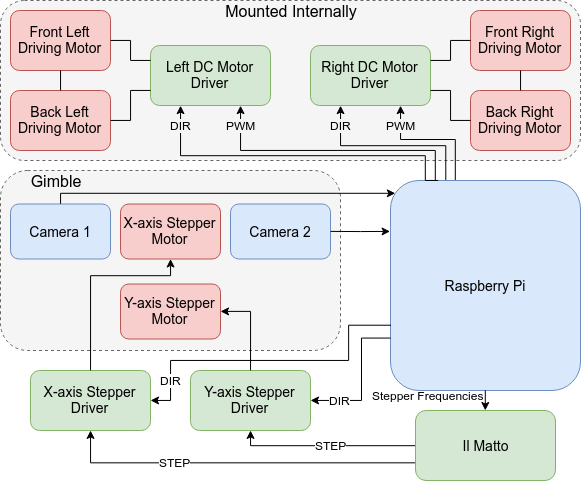
\includegraphics[width=0.9\textwidth]{Figures/hardware.png}
      \caption[Hardware Block Diagram]{Hardware Block Diagram. The red blocks are motors, green blocks are control system components, and the blue blocks are part of the image pipeline.\textcolor{red}{[MAKE IL MATTO GREEN AND RIGHT CHIP]}}
      \label{fig:hardware}
    \end{center}
\end{figure}

\section{Gimble Design}

The choice of cameras had to fulfil a very specific set of requirements. The two cameras must be same, as any differences in the images due to the cameras would reduce the quality of depth map produced by the block matching algorithm on the server. This makes the most obvious camera choice, the R-Pi camera module, unusable, as the Pi cannot use two simultaneously. The two cameras must also be able to take pictures on command from the Pi with low latency, reducing the possible options down to primarily USB webcams. Finally, they must have a high shutter speed. Any motion blur in the images will blur all the edges they contain, making them undetectable by the edge detection algorithm, and any morphing of the image while under motion due to the time it takes the shutter to pass across the entire sensor will once again reduce the quality of the depth map; a high shutter speed reduces motion blur and shutter related morphing, therefore making it essential for whenever the rover is in motion. This requirement reduces the possible cameras down to primarily dedicated computer vision cameras, however these are far outside the budget of a 3rd year project and are often too large to build a gimble for without also buying expensive motors.

\textcolor{red}{[FPV CAMERA APPENDIX?]}

Only one camera was found that fulfilled all these requirements while being cheap enough to fit within budget- the PlayStation 3 (PS3) Eye. The PS3 Eye is a camera for the PS3 to allow for games that incorporate aspects of computer vision, so it is designed with computer vision and value for money in mind. While the image quality is fairly poor, it is sufficient for the system to function reliably. 

The design of the gimble (Figure \textcolor{red}{[GIMBLE PICS]}) has considerable impact on the 3D environment the system produces. As mentioned in Section \ref{subsection:depth}, the closer the cameras are to parallel with each other, the less the images have to be rectified before the depth map is generated. Similarly, the stability of the gimble is very important, as any vibrations will cause inconsistency in the alignment of the cameras, leading to inaccurate depth maps. This led to the chosen design where the X-axis motor is located centrally, between the cameras, to balance the weight around the rotational axis of the y-axis motor. The 3D-printed part the cameras are attached to is also stabilised through mountings on both sides of the x-axis motor, using a ball bearing on the side not driven by the motor. Another important aspect of the gimble design is the distance between the camera lenses. The further apart the two cameras are, the closer distance objects will be in the depth map. Ideally we would want to match the interpupillary distance of human eyes (63mm on average \cite{dodgson2004variation}), so objects in the 3D environment appear as close as they would were the user standing in the place of the robot. However, with the X-axis motor located centrally, it is not possible to produce that distance between the camera lenses. The inter-lens distance in the final design is 120mm, as this is the closest distance possible without reducing the stability of the gimble. While not ideal, it simply results in objects appearing closer in the depth map than they actually are and a longer distance from the cameras where an object is too close for a distance to be calculated (the cameras are "cross-eyed" if you will).

\section{Image Pipeline}

As can be seen in Figure \ref{fig:system}, the rover takes a picture with both cameras, abstracts those images, then sends that data off as a single combined packet to the server. While Chapter \ref{chapter:abstract} discussed the abstraction process as a single step that produces a full abstraction with both edges and spaces filled with colour, this does not reflect the implementation utilized in the full system. As previously mentioned, the final step of filling the spaces in the edge detected image using the selected seed points and average colours is done on the server. Also, only one of the two images needs colour information at all, as the edges are the only part of the abstraction required to produce the server depth maps; the colours are to be used as a texture on the 3D environment this produces, and therefore only one set is required. Therefore, the data packets being sent to the server are made up of 2 bitmaps of the edge detected images and a set of seed points with their corresponding colours for one of the images.

Attempts to implement this process on a single thread on the Pi, as tested successfully on a laptop, either crashed the Pi or would produce a frame rate of around 1fps; the Pi's resources are not even close to adequate. To combat this, both pipelining and parallelism were utilized to make better use of the Pi's quad core processor (Figure \ref{fig:threads}), and compromises were made in the quality of the abstractions to reduce the workload.

\begin{figure}[H]
    \begin{center}
      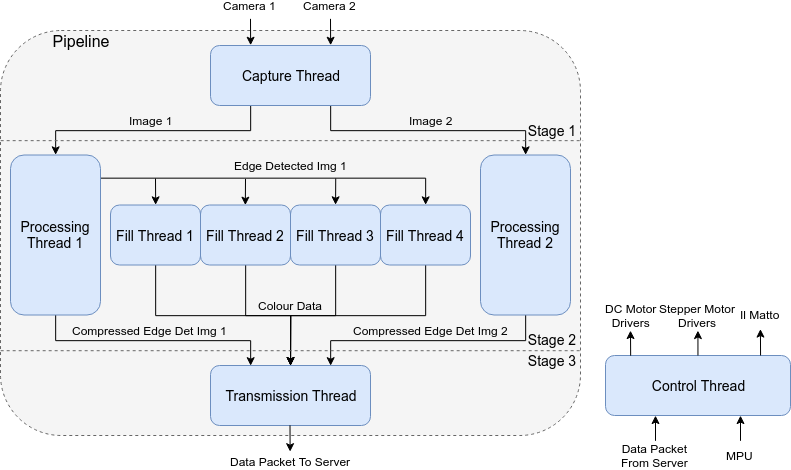
\includegraphics[width=1\textwidth]{Figures/Threads.png}
      \caption[Raspberry Pi Threading Block Diagram]{Raspberry Pi Threading Block Diagram.}
      \label{fig:threads}
    \end{center}
\end{figure}

\subsection{Communications}
\label{Subsection:comms}

\section{Control System}